%
% $RCSfile: hierarchical_algorithm.tex,v $
%
% Copyright (C) 2002-2008. Christian Heller.
%
% Permission is granted to copy, distribute and/or modify this document
% under the terms of the GNU Free Documentation License, Version 1.1 or
% any later version published by the Free Software Foundation; with no
% Invariant Sections, with no Front-Cover Texts and with no Back-Cover
% Texts. A copy of the license is included in the section entitled
% "GNU Free Documentation License".
%
% http://www.cybop.net
% - Cybernetics Oriented Programming -
%
% http://www.resmedicinae.org
% - Information in Medicine -
%
% Version: $Revision: 1.1 $ $Date: 2008-08-19 20:41:07 $ $Author: christian $
% Authors: Christian Heller <christian.heller@tuxtax.de>
%

\subsection{Hierarchical Algorithm}
\label{hierarchical_algorithm_heading}
\index{Hierarchical Algorithm}

Of course, algorithms, workflows and other activities over time can be
structured hierarchically as well.

\begin{figure}[ht]
    \begin{center}
        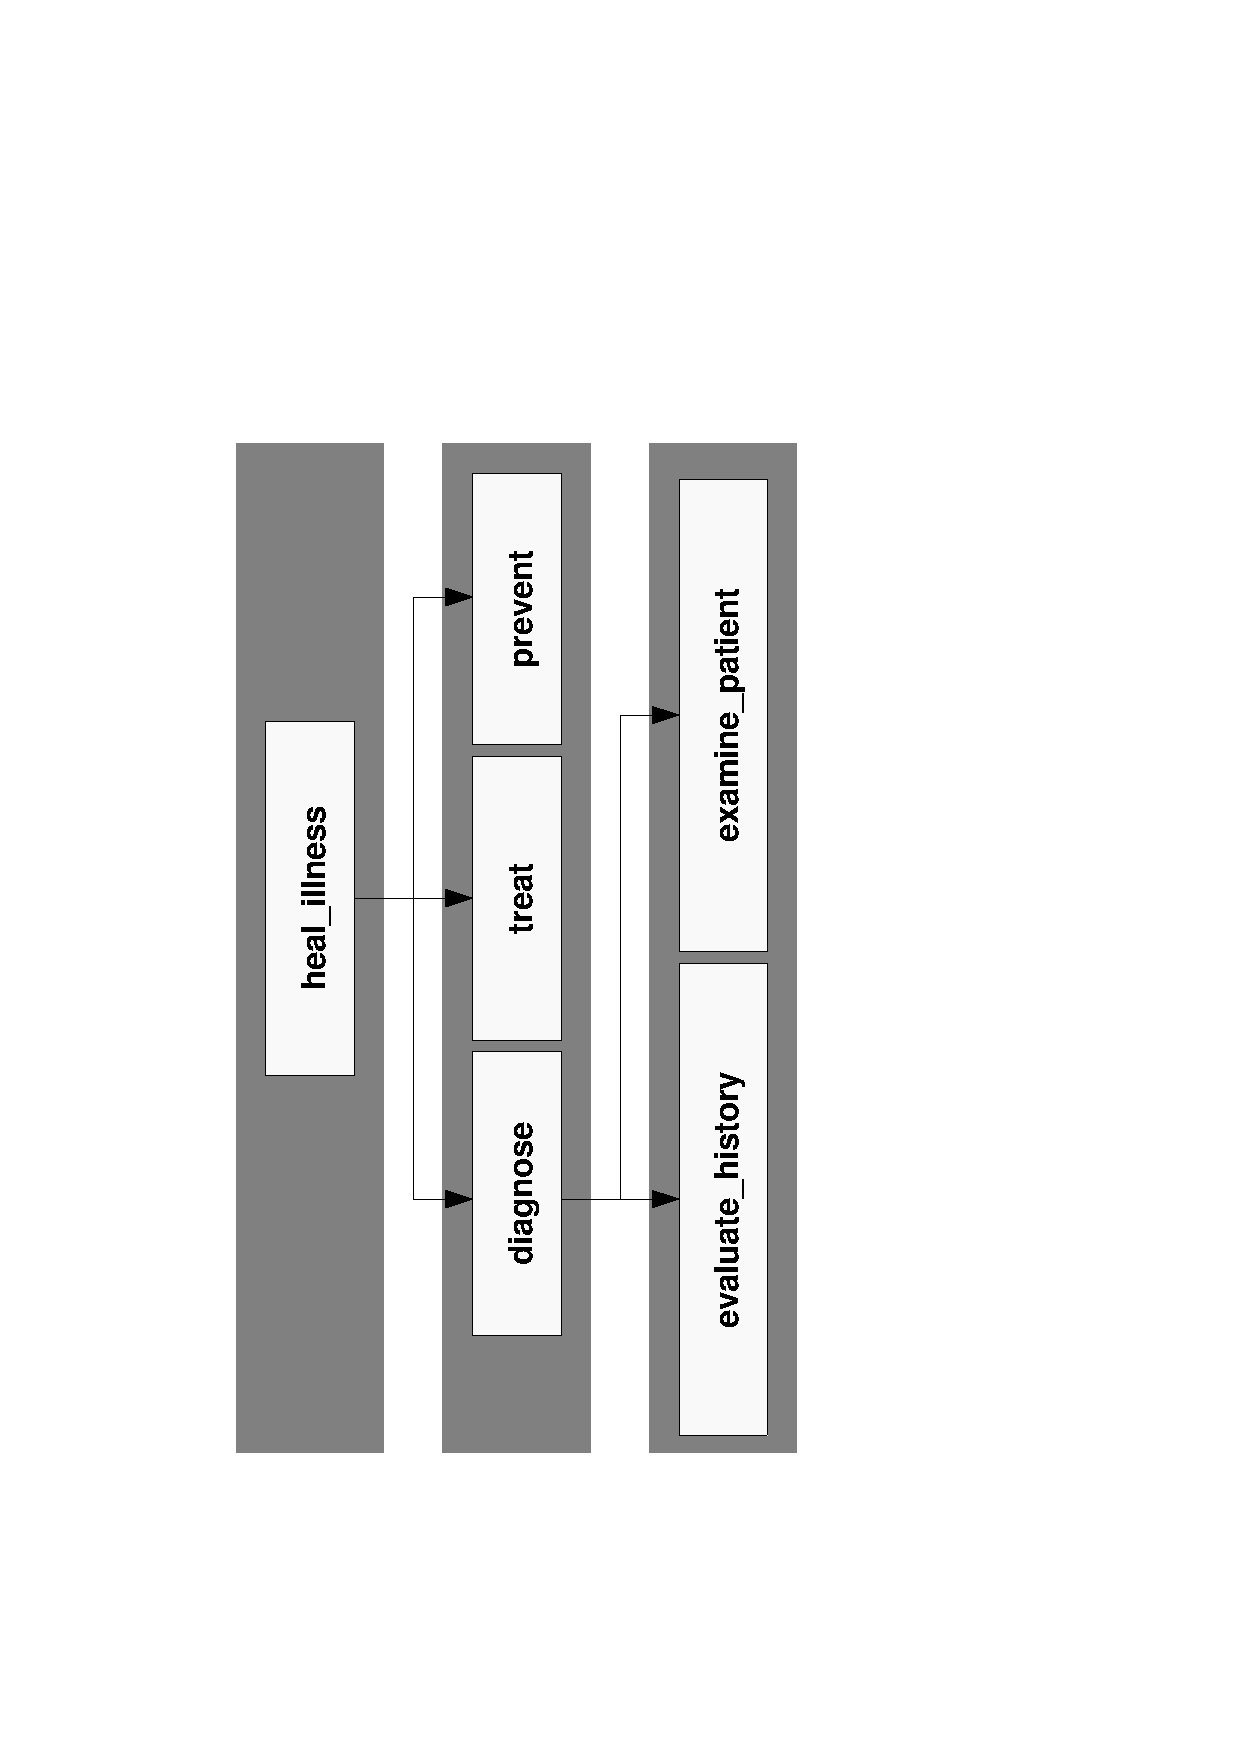
\includegraphics[scale=0.3,angle=-90]{graphic/algorithm.pdf}
        \caption{\emph{Heal Illness} as Hierarchical Algorithm, taken from Medicine}
        \label{algorithm_figure}
    \end{center}
\end{figure}

To stick with the domain of medicine: A \emph{Medical Doctor}'s (MD) activity
is to \emph{Heal an Illness}. Part processes the MD has to carry out commonly
are to \emph{Diagnose}, to \emph{Treat} and to \emph{Prevent} an illness
(figure \ref{algorithm_figure}). Further structurings are possible. To the
process of diagnostics belong activities like \emph{Evaluate History} or
\emph{Examine Patient}.
